\section{静摩擦是可调约束}
静摩擦力在不超过极限的范围内随外部作用调整，基本条件为$|f|\le\mu_sN$，而不是$f=\mu_sN$。求平衡时先写方程得到所需摩擦，再把它和允许范围比较。仅当已经说明“将滑动”或“临界平衡”，且判断了滑动趋势，才能在对应接触点取等号。多个接触点一般不会同时达到极限。

滑动摩擦$f=\mu_kN$的方向由接触处相对速度决定。对于转动物体，接触处速度包含质心平移和绕质心转动两部分；只看质心向哪边移动不足以定摩擦。静摩擦也可能帮助物体获得转动，不能把它固定理解成阻碍质心运动的力。

可把法向和摩擦合成为全反力$\boldsymbol R=N\boldsymbol n+f\boldsymbol t$。令它与法线夹角为$\varphi$，则$|\tan\varphi|=|f|/N\le\mu_s$。摩擦角$\varphi_m=\arctan\mu_s$给出允许方向锥。求解后全反力若落在锥外，说明该接触无法静止；落在边界上才是极限。

\fig{fig:s3:cone}{全反力的端点落在摩擦锥内；边界才对应极限}{\begin{tikzpicture}

\draw[world](-2,0)--(2,0);\fill[blue!8](0,0)--(-1.2,2.4)--(1.2,2.4)--cycle;\draw[guide](0,0)--(-1.2,2.4);\draw[guide](0,0)--(1.2,2.4);\draw[force](0,0)--(0,2)node[left]{$N$};\draw[force](0,0)--(.7,0)node[below]{$f$};\draw[force,blue](0,0)--(.7,2)node[right]{$\bm R$};\draw[guide](.7,0)--(.7,2)--(0,2);\draw(0,.9)arc(90:63.435:.9);\node at(.38,1.14){$\varphi_m$};\node at(4,1.7){$|f|\le\mu_sN$};\node at(4,1){$\tan\varphi_m=\mu_s$};
\end{tikzpicture}}

图\ref{fig:s3:cone}把支持力和可调静摩擦合成为全反力。合力方向必须落在摩擦角限定的允许范围内；只有边界方向对应极限静摩擦。由平衡方程反求反力后，检查其方向是否仍在范围内，才完成可实现性判定。

\subsection{分布支持力的作用点与倾覆边界}
重$G$的矩形物块底宽$b$，受高$h$处水平推力$F$，地面静摩擦系数$\mu$。底面接触压强可沿位置变化，不能总把支持力画在底面中点。若物块尚静止，竖直平衡给$N=G$，水平平衡给$f=F$；对底面中心取矩，向右推力的顺时针力矩$Fh$需由支持力作用点向右偏移$e$来抵消，所以
\[
Ge=Fh,\qquad e=\frac{Fh}{G}.
\]
图\ref{fig:s3:contactcenter}中支持力的作用点必须位于实际底面$-b/2\le e\le b/2$。支持力总量尚为正并不保证接触分布可实现，作用点越出底面同样意味着原平衡不存在。
\fig{fig:s3:contactcenter}{底面支持力作用点随水平推力向边缘移动}{\begin{tikzpicture}[scale=.88]\draw[world](-1.5,0)rectangle(1.5,2.5);\draw[world](-2,0)--(2,0);\draw[force](-1.5,1.8)--(-.2,1.8)node[above]{$F$};\draw[force](0,1.25)--(0,.3)node[right]{$G$};\draw[force](.9,0)--(.9,1)node[right]{$N$};\draw[force](.9,0)--(-.4,0)node[below]{$f$};\draw[dim](0,-.6)--(.9,-.6)node[midway,below]{$e$};\draw[dim](-2,0)--(-2,1.8)node[midway,left]{$h$};\end{tikzpicture}}
滑动边界由$F_s=\mu G$给出，倾覆边界由$e=b/2$给出$F_t=Gb/(2h)$。从$F=0$缓慢增加，先达到的较小值决定先滑还是先翻：$\mu<b/(2h)$先滑，$\mu>b/(2h)$先翻，相等时两约束同时达到边界。力的高度改变力矩而不改变总支持力，因而只写$f\le\mu G$会漏掉倾覆失稳。

若推力还含竖直分量，就应重新写$N$及外力矩，不能把上述阈值直接照搬。接触底面若为曲面或只在两个点支承，允许作用点集合也不同。对于两个支点$A,B$，由合支持力的作用点反求两支反力，$N_A+N_B=N$、$N_Bb=N(e+b/2)$；当某一反力降到零时，正是接触区缩减为另一支点的边界。

这里“支持力移到边缘”是对分布压力合力的描述，刚体尚未倾倒时并没有凭空多出一个真实支点。进入绕边缘转动后，原来的静力方程只提供临界初态，后续应加入角加速度和转动惯量。先用静力判别边界、再按新约束建立运动方程，可避免把临界结论无限延伸到全过程。

\section{临界状态与接触切换}
滑动临界由$|f|=\mu N$描述，翻倒临界由支持力作用线到达支承边缘或某一支点反力降为零描述，脱离则由$N=0$描述。这三种条件不同，可能由其中一种先发生。逐渐增大外力或倾角时，应求每一种候选临界值，再比较哪个最先达到。

均匀长方体放在斜面上是典型例子。静止所需$f/N=\tan\theta$，滑动角满足$\tan\theta_s=\mu$；重力作用线通过下边缘时，倾覆角满足$\tan\theta_t=a/b$，其中$a$是沿斜面底边、$b$是法向高度。因此$\mu<a/b$时先滑，$\mu>a/b$时先翻。用同一个“临界”一词代替不同物理条件，会把状态边界混为一谈。

\fig{s3deep:tilt}{下坡边缘与重心竖线的关系决定倾覆，而非摩擦是否达到上限}{\begin{tikzpicture}

\begin{scope}[rotate=25]
\draw[world](-.7,0)--(3.1,0);\draw[world](0,0)rectangle(2,2.5);\fill(0,0)circle(2pt)node[below]{$A$};\fill(1,1.25)circle(2pt)node[above]{$C$};\draw[dim](0,-.6)--(2,-.6)node[midway,below]{$a$};\draw[dim](2.5,0)--(2.5,2.5)node[midway,right]{$b$};
\end{scope}
\draw[guide](0,0)--(4,0);\draw[force](.378,1.556)--(.378,-.2)node[right]{$G$};\draw[dim](0,-1.2)--(.378,-1.2)node[midway,below]{$d$};\node[align=left]at(6.7,1.4){$d=\frac a2\cos\theta-\frac b2\sin\theta$\\$d=0$：重力线通过 $A$\\$\tan\theta=\mu$：摩擦达到上限};
\end{tikzpicture}}
图\ref{s3deep:tilt}中质心相对下坡角 $A$ 的水平坐标就是 $d$。$d>0$ 时重力竖线仍落在底面范围内；$d=0$ 时到达边缘；$d<0$ 时维持原构型需要底面之外的支持点。与此独立，摩擦要满足 $\tan\theta\le\mu$。求出两种边界后，比较从初态出发先遇到哪一条，才得到失稳类型。


\subsection{摩擦不等式给出的参数区间}
设由平衡式求得$f=aF+bG$、$N=cF+dG$，应先限制$N\ge0$，再用$-\mu N\le f\le\mu N$分别给出两个线性不等式。若摩擦方向事先未知，保留绝对值比凭直觉固定向左或向右更可靠。解出的区间两端可能对应相反的滑动趋势，不能只检查其中一个端点。

静摩擦系数趋零时，所需切向力必须同时趋零，否则该状态不可能保持。静摩擦系数很大时，物体也仍可能先发生倾覆、绳松弛或接触脱离。摩擦条件只限制接触切向分量，不能保证结构在任意外力下完整存在。把所有失败都归结为“摩擦不够”会忽略其他约束边界。

多点摩擦题中可把某一摩擦作为参数，解出其余反力，再由每个接触点的不等式取交集。如果交集非空，存在平衡；如果交集只剩一个点，才得到唯一静力解；若为空，则假设的接触状态不可能。这样的区间解比任意选一个数更完整，也揭示题目是否缺少变形条件。

\fig{fv:s3:interval}{平衡所需摩擦随外力改变，正负上限分别对应两种滑动趋势}{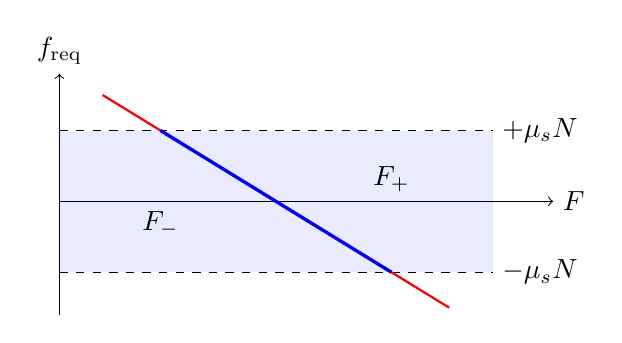
\begin{tikzpicture}[x=1.1cm,y=.9cm]
\fill[blue!8](0,-1)rectangle(5,1);\draw[->](0,0)--(5.7,0)node[right]{$F$};\draw[->](0,-1.6)--(0,1.8)node[above]{$f_{\rm req}$};
\draw[dashed](0,1)--(5,1)node[right]{$+\mu_sN$};\draw[dashed](0,-1)--(5,-1)node[right]{$-\mu_sN$};
\draw[red,thick](.5,1.5)--(4.5,-1.5);\draw[blue,very thick](1.167,1)--(3.833,-1);
\node[below]at(1.167,0){$F_-$};\node[above]at(3.833,0){$F_+$};
\end{tikzpicture}}
图\ref{fv:s3:interval}先由平衡方程求带符号的 $f_{\rm req}(F)$，再检查它是否落在允许带 $[-\mu_sN,\mu_sN]$内。蓝色线段对应整个可平衡区间，只有两端才达到极限摩擦。穿过横轴时摩擦方向改变，但物体仍可静止。若 $N$也随 $F$改变，允许带的边界会变成曲线或斜线，应联立完整不等式，不能沿用固定宽度的示意带。


\subsection{斜面拉力的上下界与摩擦反向}
静摩擦方向未知时，应把它作为有向未知量保留。图\ref{fig:s3:inclineinterval}中物体重$G$，斜面倾角$\theta$，拉力$F\ge0$与上坡方向夹角为向外的$\delta$，静摩擦系数$\mu$。沿上坡取切向正方向、离开斜面取法向正方向，设有向摩擦$f$向上为正，则
\[
F\cos\delta+f-G\sin\theta=0,\qquad
N+F\sin\delta-G\cos\theta=0.
\]
故$f=G\sin\theta-F\cos\delta$、$N=G\cos\theta-F\sin\delta$。拉力增大时既改变所需切向力，又减小可提供的法向反力，不能先把$N$固定为$G\cos\theta$。

\fig{fig:s3:inclineinterval}{同一拉力改变切向平衡和法向约束}{\begin{tikzpicture}[scale=.88]\begin{scope}[rotate=25]\draw[world](-.5,0)--(4.5,0);\draw[world](1.3,.05)rectangle(2.3,.85);\draw[force](1.8,.45)--(3.4,1.25)node[right]{$F$};\draw[force](1.8,.05)--(1.8,1.45)node[above]{$N$};\draw[force](1.8,.05)--(2.9,.05)node[below]{$f$};\draw[guide](2.3,.45)--(3.5,.45);\node at(2.9,.72){$\delta$};\end{scope}\draw[force](1.441,1.1685)--(1.441,-.65)node[right]{$G$};\node at(3.8,-.45){$f$按上坡为正};\end{tikzpicture}}
先取$\mu>0$、$0\le\delta<\arctan(1/\mu)$，保证下面两个分母均为正。将$-\mu N\le f\le\mu N$展开，分别得到
\[
F(\cos\delta-\mu\sin\delta)\ge G(\sin\theta-\mu\cos\theta),
\]
\[
F(\cos\delta+\mu\sin\delta)\le G(\sin\theta+\mu\cos\theta).
\]
因此允许范围是
\[
\max\!\left(0,\frac{G(\sin\theta-\mu\cos\theta)}{\cos\delta-\mu\sin\delta}\right)
\le F\le
\frac{G(\sin\theta+\mu\cos\theta)}{\cos\delta+\mu\sin\delta},
\]
还须与$N\ge0$给出的范围取交集。下界为正时对应物体将下滑、摩擦向上达到极限；上界对应将上滑、摩擦向下达到极限。区间内部摩擦可以经过零并反向，而物体始终静止。若$\delta=0$，恢复$G(\sin\theta-\mu\cos\theta)\le F\le G(\sin\theta+\mu\cos\theta)$；$\mu\to0$时区间收缩到无摩擦平衡值，检查一致。

当$\cos\delta-\mu\sin\delta\le0$时，不能继续按上述方向除法；应回到未除法的不等式，根据系数的零值或负号重新判断。这也是自锁题中分母变号必须单独讨论的原因。

\section{自锁的力学含义}
自锁指在给定施力方向和接触构型下，增大外力也同步增加了可提供的约束反力，使静摩擦始终足以阻止指定滑动。它不是摩擦系数无限大，也不表示物体对任意方向的力都不动。若外力改变接触点、造成离地或破坏材料，理想自锁模型便失效。

例如以向下夹角$\alpha$推水平面物块，法向力为$G+F\sin\alpha$，所需水平摩擦为$F\cos\alpha$。当$\cos\alpha-\mu\sin\alpha\le0$时，任意$F\ge0$都满足静摩擦条件；否则超过有限阈值会滑动。自锁条件来自不等式中$F$的系数，不能只把$F$趋于无穷后忽略已有的接触约束。

\fig{s3deep:lock}{向下推力同时增大滑动需求与摩擦上限}{\begin{tikzpicture}

\begin{scope}
\draw[world](-1,0)--(2.5,0);\draw[world](0,0)rectangle(1.3,1);\draw[force](-.7,1.8)--(.4,.7)node[pos=0,left]{$F$};\draw[force](.65,0)--(.65,1.5)node[right]{$N$};\draw[force](.65,.5)--(.65,-.8)node[right]{$G$};\draw[force](0,0)--(-1,0)node[left]{$f$};\draw[guide](-.7,1.8)--(.6,1.8);\draw(-.2,1.8)arc(0:-45:.5);\node at(0,1.6){$\alpha$};
\end{scope}
\begin{scope}[xshift=5cm]
\draw[axis](0,0)--(3.6,0)node[right]{$F$};\draw[axis](0,0)--(0,3.1)node[above]{切向力};\draw[blue,thick](0,.7)--(3.1,2.56)node[right]{$\mu(G+F\sin\alpha)$};\draw[red,thick](0,0)--(3.1,1.55)node[right]{$F\cos\alpha$};\node[left]at(0,.7){$\mu G$};\node at(1.7,-.7){自锁时上限斜率不小于需求斜率};
\end{scope}
\end{tikzpicture}}
图\ref{s3deep:lock}右图把需求和上限同时画成 $F$ 的函数。若上限的斜率 $\mu\sin\alpha$ 不小于需求斜率 $\cos\alpha$，两线不会相交，指定方向的滑动被锁住；反之两线在有限 $F_c$ 处相交。图示只检验滑动，物体若有有限底面，还需像图\ref{fig:s3:contactcenter}那样检查支持力作用点，不能用自锁结论排除倾覆。


细杆、抽屉及夹持问题中，外力还通过力矩放大法向力。应同时使用力平衡、力矩平衡和摩擦锥条件。有时把支承全反力的作用线延长到绳线交点，就能几何地看出载荷落在哪一区间可被锁住；代数推导则给出精确阈值。

\subsection{夹持、自锁与施力方向的优化}
若施力总大小受限，允许向斜面外侧提拉可减少法向力及摩擦，从而改善上坡能力；但法向力不能被减到负值。设外力相对上坡方向向外偏$\delta$，上坡能力含$F(\cos\delta+\mu\sin\delta)$，其最大值在$\delta=\arctan\mu$，前提是此时$N\ge0$。若只允许向面内推，最优方向一般退到约束边界，结果不同。

施力点的位置也会改变自锁。高处横向拉一根受绳约束的杆，拉力既直接要求地面摩擦，又通过上端绳张力改变法向力。关于底端的力矩式给出张力随$F$的增大比例，再代回法向方程才能判断是否自锁。跳过力矩、只把$N$当作重力，会完全丢失高度$h$的影响。


\section{多接触系统与不定静力}
刚体平面平衡只有三个独立标量方程。如果未知接触分量超过这个数，静摩擦不等式通常只能给范围，不能唯一给出各点摩擦。这是模型信息不足，并不意味着可以任意多写一个$f=\mu N$。若题目没有给出临界状态或变形关系，应把结果写成参数族和可行区间。

对滚动与滑动的切换，可先按纯滚动速度约束求所需摩擦，再检验它是否在静摩擦锥内；若超出，改为滑动摩擦并重新确定接触相对速度方向。缓慢改变装置也不意味着每一个接触点都在滑动，特别是圆柱同时接触墙与板时，需要检验两处纯滚动是否几何相容。

\subsection{两处粗糙接触怎样给出可行区间}
均匀梯子重$G$，下端$A$在粗糙水平地面，上端$B$靠粗糙竖墙，杆与水平面夹角$\theta$。如图\ref{fig:s3:ladderfamily}，墙对梯子的法向力$H$向左，墙摩擦$j$取向上为正，地面摩擦$f$取向右为正。整体平衡为
\[
f=H,\qquad N+j=G,\qquad
jL\cos\theta+HL\sin\theta=\frac{GL}{2}\cos\theta.
\]

\fig{fig:s3:ladderfamily}{两处粗糙接触各有独立的摩擦限制}{\begin{tikzpicture}[scale=.88]\draw[world](-.4,0)--(3.6,0);\draw[world](3,0)--(3,3.7);\draw[world,line width=1.4pt](0,0)--(3,3);\node[below left]at(0,0){$A$};\node[below right]at(3,3){$B$};\draw[force](0,0)--(0,1.2)node[left]{$N$};\draw[force](0,0)--(1.2,0)node[below]{$f$};\draw[force](3,3)--(1.9,3)node[above]{$H$};\draw[force](3,3)--(3,4.1)node[right]{$j$};\draw[force](1.5,1.5)--(1.5,.35)node[right]{$G$};\node at(.8,.3){$\theta$};\end{tikzpicture}}
第三式约去$L\cos\theta$后，得$j=G/2-H\tan\theta$，再由竖直平衡得$N=G/2+H\tan\theta$。这时$H$仍是参数，必须同时满足
\[
H\ge0,\quad N\ge0,\quad H\le\mu_A N,
\quad |G/2-H\tan\theta|\le\mu_BH.
\]
例如$\theta=45^\circ$、$\mu_A=\mu_B=1/2$时，地面条件给$H\le G/2$；墙条件拆成$G/2-H\le H/2$及$G/2-H\ge-H/2$，给$G/3\le H\le G$。取交集，$G/3\le H\le G/2$，并有$0\le j\le G/6$。区间下端是墙摩擦达到极限，区间上端是地面摩擦达到极限，两者没有同时取满。

\fig{s3deep:intersection}{两处摩擦条件分别给区间，平衡存在性由交集决定}{\begin{tikzpicture}

\foreach \yy/\lab in {2/地面条件,1/墙面条件,0/共同可行区间}{\draw[axis](0,\yy)--(6.6,\yy);\node[left]at(0,\yy){\lab};}
\draw[blue,line width=2pt](0,2)--(3,2);\draw[red,line width=2pt](2,1)--(6,1);\draw[green!50!black,line width=3pt](2,0)--(3,0);\draw[guide](2,-.3)--(2,2.5);\draw[guide](3,-.3)--(3,2.5);\node[below]at(2,-.3){$G/3$};\node[below]at(3,-.3){$G/2$};\node[below]at(6,-.3){$G$};\node[right]at(6.6,0){$H$};\node[above]at(2,2.6){墙临界};\node[above]at(3.5,2.6){地面临界};
\end{tikzpicture}}
图\ref{s3deep:intersection}显示两处的边界发生在不同 $H$ 值：在 $H=G/3$ 处只有墙达到极限，在 $H=G/2$ 处只有地面达到极限；交集内部两处都未取满。若要继续判定实际反力落在哪一点，须增加接触形变或加载信息。


所以这组理想刚体条件能证明平衡存在，却不能唯一确定两处摩擦。若一开始同时令$f=\mu_AN$、$j=\mu_BH$，就额外强加了题目没有给出的临界关系，甚至会把本来存在的平衡误判为不存在。真实反力分配还可由接触弹性与加载历史决定；若题目只问能否静止或参数范围，可行区间本身就是完整答案。

\subsection{滚动接触的方向与状态判别}
圆柱与运动平面接触时，设质心速度为$\boldsymbol V$、角速度$\boldsymbol\omega$、接触点相对质心位置为$\boldsymbol r$，则接触处相对速度为$\boldsymbol V+\boldsymbol\omega\times\boldsymbol r-\boldsymbol U_{\rm surface}$。先计算它的切向分量，再决定动摩擦方向。相对速度为零时改用静摩擦范围，而不能把原来的动摩擦方向机械延续。

一个圆柱同时接触两面时，两处无滑动条件未必相容。应先把两条件和法向不穿透条件共同代入速度关系；若除了静止外无解，就说明移动边界下至少有一处滑动。若题目只说“缓慢”而没有给加载方式、摩擦系数或接触状态，单一的先顺时针后逆时针结论通常无法由几何保证。

当法向反力中出现形如$1-\mu_1\mu_2$或某个三角组合的分母时，分母过零不是支持力可以直接变成负数，而是接触分支失效、形成自锁或需要新的运动模式的信号。应回到未除法的方程核对符号，再寻找$N=0$、相对速度变号或静摩擦达到极限的切换事件。


\subsection{接触间隙和滚动条件的相容性}
普通接触既不能穿透也不能拉住物体。若两表面的间隙为$d$，法向反力为$N$，理想单向接触要求$d\ge0$、$N\ge0$，且$Nd=0$：有正间隙必无接触力，有正接触力则间隙必须为零。$d=N=0$只是切换候选状态，还需看接下来两面是靠近还是分离；有碰撞时另需冲量关系。这些条件不能用“支持力取正”一句话替代全部状态判断。

无滑动条件还要和几何约束相容。图\ref{fig:s3:twocontacts}中半径$R$的圆柱同时接触固定竖墙及向右以$U$运动的水平板，且圆心位置保持不变。取逆时针角速度$\omega$为正，底部材料点$A$的速度为$\omega R$向右，右侧点$B$的速度为$\omega R$向上。若两处都粘着，分别要求
\[
\omega R=U\quad\hbox{（底部）},\qquad
\omega R=0\quad\hbox{（墙面）}.
\]

\fig{fig:s3:twocontacts}{固定圆心下两处无滑动条件不能同时适应移动底板}{\begin{tikzpicture}[scale=.88]\draw[world](-.4,0)--(4,0);\draw[world](3,0)--(3,3.2);\draw[world](1.6,1.4)circle(1.4);\fill(1.6,1.4)circle(2pt)node[left]{$C$};\fill(1.6,0)circle(2pt)node[below]{$A$};\fill(3,1.4)circle(2pt)node[right]{$B$};\draw[guide](1.6,0)--(1.6,1.4)--(3,1.4);\draw[flow](1.6,.15)--(2.6,.15)node[above]{$\omega R$};\draw[flow](2.85,1.4)--(2.85,2.4)node[left]{$\omega R$};\draw[flow](.2,-.7)--(1.3,-.7)node[right]{$U$};\node at(.2,2.8){$\omega>0$};\end{tikzpicture}}
当$U\ne0$时两条件矛盾，至少有一处滑动。若墙面粘着，$\omega=0$，底板相对柱底向右滑动，底板对柱的摩擦向右；若底部粘着，$\omega=U/R>0$，柱的右侧点相对墙向上滑动，墙摩擦向下。随后应对候选分支分别列受力和力矩方程，检验另一处所需静摩擦是否足够。边界移动得很慢并不能消除这种运动学矛盾，也不能预先保证两处摩擦都等于极限值。

\section{受力优化与轨迹约束}
若外力方向可以选择，可把其沿运动方向的分量用于克服重力和摩擦，垂直分量则改变法向力。最优方向来自这两种作用的共同效果。必须说明施力装置的能力限制是总力不超过某值，还是仅某一分量受限；不同限制对应不同优化问题。

物体在斜面上被平行斜面的轻绳缓慢牵引时，速度方向沿轨迹切线，绳力沿指向固定滑轮的径向，滑动摩擦反向沿切线。
取滑轮所在点为极点 $O$，以斜面内的下坡方向为极角零方向。
令物体位置为 $(\rho,\varphi)$，实际速度与向外径向 $\bm e_\rho$ 的有向夹角为 $\psi$。
图\ref{s3:trajectory-directions}中，沿轨迹的单位切向量为
$\bm t=\cos\psi\,\bm e_\rho+\sin\psi\,\bm e_\varphi$。

\fig{s3:trajectory-directions}{左图把轨迹切线分解到极坐标方向；右图在斜面内按实际速度确定摩擦方向}{\begin{tikzpicture}[scale=.85]
\begin{scope}
\fill(0,0)circle(2pt)node[below left]{$O$};
\draw[flow](0,0)--(3.3,0)node[below]{下坡};
\draw[guide](0,0)--(2.6,1.5)node[midway,above left]{$\rho$};
\draw[->](.8,0)arc(0:30:.8)node[midway,right]{$\varphi$};
\fill(2.6,1.5)circle(2pt)node[right]{$P$};
\draw[flow](2.6,1.5)--(3.55,2.05)node[right]{$\bm e_\rho$};
\draw[flow](2.6,1.5)--(2.05,2.45)node[above]{$\bm e_\varphi$};
\draw[flow,blue](2.6,1.5)--(2.05,.55)node[left]{$\bm v=v\bm t$};
\draw[->](3.033,1.75)arc(30:-120:.5);\node at(3.15,1.05){$\psi$};
\end{scope}
\begin{scope}[xshift=6cm]
\fill(0,0)circle(2pt)node[below right]{$P$};
\draw[force](0,0)--(-1.5,-.866)node[below]{$-T\bm e_\rho$};
\draw[force](0,0)--(1.2,0)node[right]{$mg\sin\alpha$};
\draw[force](0,0)--(.5,.866)node[above]{$-\mu N\bm t$};
\node at(0,-1.6){$N=mg\cos\alpha$};
\end{scope}
\end{tikzpicture}}

设斜面倾角为 $\alpha$，滑动摩擦系数为 $\mu>0$。牵引力平行斜面时，
$N=mg\cos\alpha$。下坡方向在极坐标中为
$\cos\varphi\,\bm e_\rho-\sin\varphi\,\bm e_\varphi$。
沿 $\bm e_\varphi$ 投影，绳力没有这一方向的分量，准静态平衡给出
\[
 -mg\sin\alpha\sin\varphi-\mu mg\cos\alpha\sin\psi=0,
 \qquad \sin\psi=-\frac{\tan\alpha}{\mu}\sin\varphi.
\]
这一步从受力确定了切线方向，但还要依据收绳或放绳选择 $\cos\psi$ 的符号；
例如向滑轮靠近时 $\dot\rho<0$，应取 $\cos\psi<0$。
随后才由速度分解
\[
 \dot\rho=v\cos\psi,\qquad \rho\dot\varphi=v\sin\psi
\]
消去速率，得到轨迹方程
\[
 \frac{\dd\rho}{\dd\varphi}=\rho\cot\psi(\varphi)
 \quad (\dot\varphi\ne0).
\]
沿给定初始位置积分，才能确定具体轨迹；若 $\dot\varphi=0$，应回到分量式单独处理径向运动。
还须检查 $|\sin\psi|\le1$，以及径向平衡给出的
$T=mg\sin\alpha\cos\varphi-\mu mg\cos\alpha\cos\psi\ge0$。
不满足这些条件时，所假设的缓慢、绳绷紧运动不能维持。
这里“缓慢”表示可忽略惯性，仍须由实际速度确定摩擦，不能先假定轨迹为直线。

\section{准静态运动中的摩擦做功}
准静态表示惯性项相对外力可以忽略，并不表示没有位移、速度或能量耗散。物体缓慢滑过粗糙面时，动摩擦仍可做有限负功，外力的输入功主要转化为重力势能或内能。把每一时刻当作力平衡，是求外力的方法；计算全过程功时仍要沿实际路径积分。

摩擦对物体所做的功和系统机械能损失也要区分。下表面运动时，静摩擦可以对上物体做正功；滑动摩擦对某个物体也未必总做负功，因为其方向与相对速度相反，而功使用物体对地速度。把接触的两物体记为$A,B$，令$\boldsymbol v_{\rm rel}=\boldsymbol v_A-\boldsymbol v_B$，则作用于$A$的摩擦为$\boldsymbol f_A=-\mu N\boldsymbol v_{\rm rel}/|\boldsymbol v_{\rm rel}|$，作用于$B$的力相反。两个摩擦功率相加，
\[
P_A+P_B=\boldsymbol f_A\cdot\boldsymbol v_A
-\boldsymbol f_A\cdot\boldsymbol v_B
=-\mu N|\boldsymbol v_{\rm rel}|\le0.
\]
因此系统损失机械能的速率是$\mu N|\boldsymbol v_{\rm rel}|$；某一个物体单独得到正功，并不与总耗散矛盾。这里的速度应取接触处材料点的速度；有转动时不能只代质心速度。

\fig{s3deep:power}{运动底板可对木块做正功，但两接触体的总摩擦功率为负}{\begin{tikzpicture}

\draw[world](0,0)rectangle(5,.35);\draw[world,fill=blue!6](1.4,.35)rectangle(2.8,1.3);\node at(2.1,.85){$A$};\node at(4.5,.17){$B$};\draw[flow](2.8,1.1)--(3.8,1.1)node[right]{$v_A$};\draw[flow](1,-.6)--(3.5,-.6)node[right]{$v_B>v_A>0$};\draw[force](2.1,.5)--(3.5,.5)node[right]{$f_A$};\draw[force](2.1,.15)--(.7,.15)node[below]{$f_B=-f_A$};\node[align=left]at(7.8,1){$P_A=f_Av_A>0$\\$P_B=-f_Av_B<0$\\$P_A+P_B=-\mu N(v_B-v_A)$};
\end{tikzpicture}}
图\ref{s3deep:power}中底板比木块向右运动得更快，木块相对板向左滑，所以板对木块的摩擦向右。该力对木块做正功，同时木块对底板的摩擦做更大的负功；差额才是接触处的机械能耗散。这里两接触面均作平动，故图中的速度也就是接触材料点速度。


理想纯滚动中，若支承面静止，接触点对地瞬时速度为零，静摩擦的瞬时功率为零，但它仍可能提供改变转动的力矩。若支承面本身运动，接触点对地不再静止，不能继续断言静摩擦不做功。判断功时应在图中标明所用参考系和作用点速度，避免只凭“静摩擦”名称下结论。

自锁装置能保持负载，并不意味着它可以在锁住状态连续输出功。要使其实际移动，通常需改变施力方向、降低接触正压力或解除约束。极小的速度也可能伴随从静摩擦到动摩擦的突变，因此跨越启动阈值后应重新核对运动方程，不能把临界静力关系当作随后的恒定运动关系。

在摩擦角图中，合反力位于锥内对应一段允许范围；沿某一虚位移方向讨论摩擦功，只能检验该方向的趋势。空间问题允许运动方向不止一个时，应对全部切向分量使用圆锥约束，不能分别令每个切向分量都小于$\mu N$后就认为总摩擦一定可行，因为分量合成的大小仍可能超过极限。

